\documentclass{article}


\usepackage{arxiv}

\usepackage[utf8]{inputenc} % allow utf-8 input
\usepackage[T1]{fontenc}    % use 8-bit T1 fonts
\usepackage{hyperref}       % hyperlinks
\usepackage{url}            % simple URL typesetting
\usepackage{booktabs}       % professional-quality tables
\usepackage{amsfonts}       % blackboard math symbols
\usepackage{nicefrac}       % compact symbols for 1/2, etc.
\usepackage{microtype}      % microtypography
\usepackage{lipsum}		% Can be removed after putting your text content
\usepackage{textgreek}
\usepackage{amsmath}
\usepackage{algorithm}
\usepackage{algpseudocode}
\usepackage{algpascal}
\usepackage{graphicx}
\graphicspath{ {./images/} }

\title{Replicating Sutton's $TD(\lambda)$ Algorithm}

\date{June 1st, 2019}	% Here you can change the date presented in the paper title
%\date{} 					% Or removing it

\author{
  Carlos Souza\\
  %Department of Computer Science\\
  Georgia Institute of Technology\\
  São Paulo, SP, Brazil \\
  \texttt{souza@gatech.edu} \\
}

\begin{document}
\maketitle

\begin{abstract}
\lipsum[1]
\end{abstract}


% keywords can be removed
\keywords{First keyword \and Second keyword \and More}


\section{Introduction}
\label{sec:introduction}
Temporal-difference (TD) learning is a core learning technique in modern reinforcement learning  (Sutton, 1988; Kaelbling, Littman \& Moore; Sutton \& Barto, 1998; Szepesvári, 2014).
TD learning generates good estimates for expected returns by quickly bootstrapping from other expected-return estimates. TD(\textlambda) is one of the most popular algorithms in TD learning.
It was first introduced in Sutton's article \emph{Learning to Predict by the Methods of Temporal Differences}, one of the most referenced articles in the field with over 5,000 citations.
The purpose of this paper is to discuss the results obtained by replicating Sutton's TD(\textlambda) algorithm, providing a complete description of the experiments, implementation details and outcomes.

\subsection{Background}
\label{subsec:background}
Our focus in this paper are \emph{Markov Reward Processes}.
MRPs are stochastic processes that can be described by \(\langle\mathcal{S}, p, r, \gamma\rangle\), where \(\mathcal{S}\) is the set of all possible states, \(p(s'|s)\) is the transition probability from state \(s \in \mathcal{S}\) to state \(s' \in \mathcal{S}\), \(r(s, s')\) is the reward obtained in the transition, and \(\gamma\) is the discount factor.

We will also focus on episodic MRPs, processes that contain \emph{terminal states}.
These states divide the sequences of state transitions into \emph{episodes}.
Once a terminal state is reached, the episode ends and the state is reset to its initial value.
The return at time step \(t\) is the discounted sum of all the rewards observed after this time step until the end of the episode:

\begin{equation}
    G_{t} = \sum_{i=1}^{T-t} \gamma^{i-1} R_{i+1}\label{eqn:1}
\end{equation}

where \emph{T} is the time step of the terminal state.

Our goal is to learn the state-value function $v$ that maps each state $s \in \mathcal{S}$ to the expected return:

\begin{equation}
    v(s) = \mathbb{E}\{G_{t} \mid S_{t} = s\}\label{eqn:2}
\end{equation}

One of the simplest ways to solve a MRP is using Monte Carlo methods.
These methods solve reinforcement learning problems by using experience from interactions with the environment to update their estimate $V$ of $v$ for the nonterminal state $S_{t}$ ocurring in the experience.
Monte Carlo methods wait until the end of the episode, until the full return following the visit is known, to use this value to update current estimate of the state-value function:

\begin{equation}
    V(S_{t}) \leftarrow V(S_{t}) + \alpha(G_{t} - V(S_{t}))\label{eqn:3}
\end{equation}


where $\alpha$ is the learning-rate.
The problem with Monte Carlo methods is that $G_{t}$ is only known by the end of the episode, which means these methods must wait until the end of the episode to determine the increment to $V(S_{t})$.
TD methods, in other hand, need to wait only until the next step $t + 1$.
The simplest TD method, $TD(0)$, uses the observed reward $R_{t+1}$ and the current estimate $V(S_{t+1})$ from the next time step to update value-function estimate of current state:

\begin{equation}
    V(S_{t}) \leftarrow V(S_{t}) + \alpha \underbrace{(R_{t+1} + \gamma V(S_{t+1}) - V(S_{t}))}_{\delta \text{, known as TD error}} \label{eqn:4}
\end{equation}

$TD(0)$, also called \emph{one-step TD}, is just an instance of a more general class of algorithms called $TD(\lambda)$, where $\lambda = 0$.
The general $TD(\lambda)$ unify and generalize TD and Monte Carlo methods, producing methods that have Monte Carlo at one extreme ($\lambda = 1$) and one-step TD at the other ($\lambda = 0$).
Its update rule is similar to the $TD(0)$:

\begin{equation}
    V(S_{t}) \leftarrow V(S_{t}) + \alpha (R_{t+1} + \gamma V(S_{t+1}) - V(S_{t})) \: e(S_{t})\label{eqn:5}
\end{equation}

however, it is applied to \emph{all states} accordingly to their \emph{eligibility} $e(S_{t})$.
The eligibility of a state is the degree to which it has been visited in the past.
It is a short-term memory vector that is bumped in the component correspondent to the state recently visited, then fading away in proportion to $\lambda$.
Eligibility can be updated incrementaly as:

\begin{equation}
    e(s) \leftarrow \begin{cases}
                            \gamma \lambda \: e(s) + 1 &\text{if $s =$ current state}\\
                            \gamma \lambda \: e(s) &\text{otherwise}\label{eqn:6}
    \end{cases}
\end{equation}

We can use equations (\ref{eqn:5}) and (\ref{eqn:6}) to devise $TD(\lambda)$ algorithm:

\alglanguage{pseudocode}
\begin{algorithm}
    \caption{Value-state prediction with $TD(\lambda)$}
    \begin{algorithmic}
        \State Initialize state-value function $V$ arbitrarily
        \For{$episode \gets 1,\, M$}
            \State Initialize $S$
            \State Initialize $e$ to $0$ for all $s \in \mathcal{S}$
            \For{$t \gets 1,\, T$} \Comment{For each time step $t$ in the $episode$}
                \State Observe reward $R_{t+1}$ and next state $S_{t+1}$
                \State $e(S_{t}) \gets e(S_{t}) + 1$
                \State $\delta \gets R_{t+1} + \gamma V(S_{t+1}) - V(S)$
                \State $V(s) \gets V(s) + \alpha \: \delta \: e(s)$ for all $s \in \mathcal{S}$
                \State $e(s) \gets \gamma \: \lambda \: e(s)$ for all $s \in \mathcal{S}$
                \State $S_{t} \gets S_{t+1}$
            \EndFor
        \EndFor
    \end{algorithmic}
\end{algorithm}


\subsection{Random Walk}
\label{subsec:randomwalk}
Sutton (1988) illustrates TD methods with a random-walk example, one of the simplest dynamic systems.
A bounded random walk is a Markov Reward Process.
The episodes always start in the middle state $D$.
At each time step, the walk moves to the neighbor state, either left or right, with equal probability.
The episode ends when walk reaches either extreme states $A$ or $G$.
If termination happens by reaching the extreme right ($G$), environment provides a reward of +1;
all the other rewards are zero.

\begin{figure}[t]
    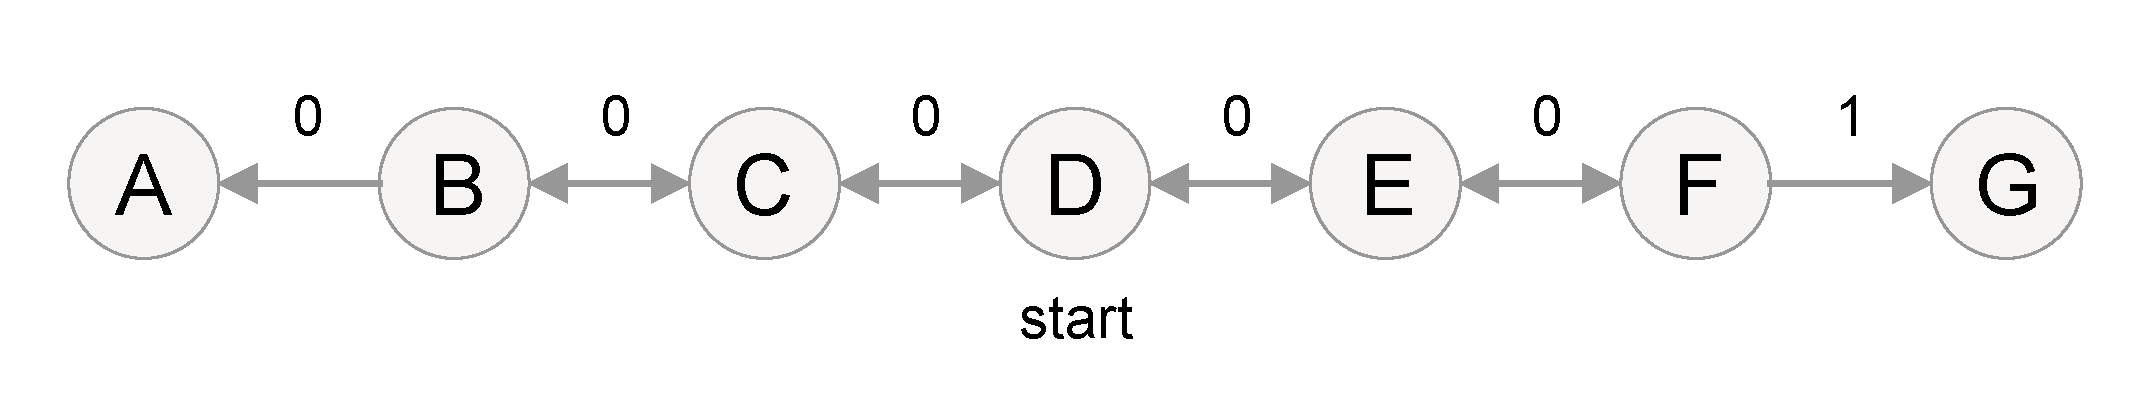
\includegraphics[scale=0.3]{random_walk.eps}
    \centering
    \caption{A bounded random walk generator used in Sutton's original paper.
    All episodes start in state $D$.
    At each time step, walk has equal probability of either moving left or right.
    Episode ends when walk reaches either $A$ or $G$.
    In case of episode terminating in $G$, +1 reward is received;
    otherwise, reward is zero.}
\end{figure}

A typical episode terminating in the extreme right might be the following state-reward sequence: $D, 0, C, 0, D, 0, E, 0, F, 0, G, 1$.
An example of a walk ending in the extreme left might be: $D, 0, C, 0, B, 0, A, 0$.
This MRP is undiscounted ($\gamma = 1$);
therefore, the true value of each state is the probability of terminating on the extreme right by starting from that specific state.
Thus, the true values from all states, from $A$ to $G$ respectively, are

\begin{equation}
    v_{true} = \Bigg[0, \frac{1}{6}, \frac{2}{6}, \frac{3}{6}, \frac{4}{6}, \frac{5}{6}, 1\Bigg]
    \centering
\end{equation}

We applied $TD(\lambda)$ algorithm to effectively predict these true values, replicating Sutton's original paper methods and results.
The following sections explain in details how we implemented the experiments, their results, and compares them with the previously published outcomes.

\section{Methods}
\label{sec:methods}
\lipsum[2]
\lipsum[3]

\section{Results}
\label{sec:results}
\lipsum[2]
\lipsum[3]

\section{Discussion}
\label{sec:discussion}
\lipsum[2]
\lipsum[3]

\section{Conclusion}
\label{sec:conclusion}
\lipsum[2]
\lipsum[3]

\section{Headings: first level}
\label{sec:headings}

\lipsum[4] See Section \ref{sec:headings}.

\subsection{Headings: second level}
\lipsum[5]
\begin{equation}
\xi _{ij}(t)=P(x_{t}=i,x_{t+1}=j|y,v,w;\theta)= {\frac {\alpha _{i}(t)a^{w_t}_{ij}\beta _{j}(t+1)b^{v_{t+1}}_{j}(y_{t+1})}{\sum _{i=1}^{N} \sum _{j=1}^{N} \alpha _{i}(t)a^{w_t}_{ij}\beta _{j}(t+1)b^{v_{t+1}}_{j}(y_{t+1})}}
\end{equation}

\subsubsection{Headings: third level}
\lipsum[6]

\paragraph{Paragraph}
\lipsum[7]

\section{Examples of citations, figures, tables, references}
\label{sec:others}
\lipsum[8] \cite{kour2014real,kour2014fast} and see \cite{hadash2018estimate}.

The documentation for \verb+natbib+ may be found at
\begin{center}
  \url{http://mirrors.ctan.org/macros/latex/contrib/natbib/natnotes.pdf}
\end{center}
Of note is the command \verb+\citet+, which produces citations
appropriate for use in inline text.  For example,
\begin{verbatim}
   \citet{hasselmo} investigated\dots
\end{verbatim}
produces
\begin{quote}
  Hasselmo, et al.\ (1995) investigated\dots
\end{quote}

\begin{center}
  \url{https://www.ctan.org/pkg/booktabs}
\end{center}


\subsection{Figures}
\lipsum[10] 
See Figure \ref{fig:fig1}. Here is how you add footnotes. \footnote{Sample of the first footnote.}
\lipsum[11] 

\begin{figure}
  \centering
  \fbox{\rule[-.5cm]{4cm}{4cm} \rule[-.5cm]{4cm}{0cm}}
  \caption{Sample figure caption.}
  \label{fig:fig1}
\end{figure}

\subsection{Tables}
\lipsum[12]
See awesome Table~\ref{tab:table}.

\begin{table}
 \caption{Sample table title}
  \centering
  \begin{tabular}{lll}
    \toprule
    \multicolumn{2}{c}{Part}                   \\
    \cmidrule(r){1-2}
    Name     & Description     & Size ($\mu$m) \\
    \midrule
    Dendrite & Input terminal  & $\sim$100     \\
    Axon     & Output terminal & $\sim$10      \\
    Soma     & Cell body       & up to $10^6$  \\
    \bottomrule
  \end{tabular}
  \label{tab:table}
\end{table}

\subsection{Lists}
\begin{itemize}
\item Lorem ipsum dolor sit amet
\item consectetur adipiscing elit. 
\item Aliquam dignissim blandit est, in dictum tortor gravida eget. In ac rutrum magna.
\end{itemize}


\bibliographystyle{unsrt}  
%\bibliography{references}  %%% Remove comment to use the external .bib file (using bibtex).
%%% and comment out the ``thebibliography'' section.


%%% Comment out this section when you \bibliography{references} is enabled.
\begin{thebibliography}{1}

\bibitem{kour2014real}
George Kour and Raid Saabne.
\newblock Real-time segmentation of on-line handwritten arabic script.
\newblock In {\em Frontiers in Handwriting Recognition (ICFHR), 2014 14th
  International Conference on}, pages 417--422. IEEE, 2014.

\bibitem{kour2014fast}
George Kour and Raid Saabne.
\newblock Fast classification of handwritten on-line arabic characters.
\newblock In {\em Soft Computing and Pattern Recognition (SoCPaR), 2014 6th
  International Conference of}, pages 312--318. IEEE, 2014.

\bibitem{hadash2018estimate}
Guy Hadash, Einat Kermany, Boaz Carmeli, Ofer Lavi, George Kour, and Alon
  Jacovi.
\newblock Estimate and replace: A novel approach to integrating deep neural
  networks with existing applications.
\newblock {\em arXiv preprint arXiv:1804.09028}, 2018.

\end{thebibliography}


\end{document}
